\documentclass[a4paper,12pt]{article} %размер бумаги устанавливаем А4, шрифт 12пунктов
\usepackage{ucs}
\usepackage{amsmath}
\usepackage{mathtext}
\usepackage{pstool}
\usepackage{color}
\usepackage{amsfonts}
\usepackage{amssymb}
\usepackage{amsthm} %proof подключаем
\usepackage{mathtools}
\usepackage[utf8x]{inputenc} % Включаем поддержку UTF8
\usepackage[russian]{babel}  % Включаем пакет для поддержки русского языка
\date{}
\author{}
\usepackage{mathrsfs}
\usepackage{graphicx} %хотим вставлять в диплом рисунки?
\usepackage{caption}
\usepackage{sidecap}
\usepackage{wrapfig}
\usepackage{pgf,tikz}
\usetikzlibrary{patterns}
\usetikzlibrary{arrows}
\usepackage{pgf, tikz}
\usepackage[left=3cm,right=2cm,
    top=2cm,bottom=2cm,bindingoffset=0cm]{geometry}
\usetikzlibrary{arrows}

\usepackage{setspace}
\graphicspath{{images/}}%путь к рисункам
\DeclareGraphicsExtensions{.pdf,.png,.jpg}

\makeatletter
\renewcommand{\@biblabel}[1]{#1.} % Заменяем библиографию с квадратных скобок на точку:
\makeatother

\newcommand{\divisible}{\mathop{\raisebox{-2pt}{\vdots}}}

\begin{document}
\begin{flushleft}
{Пособие №9}
\hfill
{\bf ``Кванторы (математические символы)''}
\end{flushleft}				

\begin{center}
{\largeТеоретический материал}
\end{center}

\newcommand{\hm}[1]{#1\nobreak\discretionary{}{\hbox{\ensuremath{#1}}}{}}
\begin{enumerate}
\item $``\in"$ - значок принадлежности, например, $a \in A$, т.е. элемент (a) принадлежит множеству A; $``\notin "$ - не принадлежит
\item $``\varnothing "$ - пустое множество, т.е. множество, не содержащее никаких элементов
\item $\mathbb N$ - множество натуральных чисел; $\mathbb Z$ - множество целых чисел; $\mathbb R$ - множество действительных чисел; $\mathbb Q$ - множество рациональных чисел
\item запись исключения элемента из множества $A\setminus {a}$, например, множество $A=[-1;1]$ - отрезок, $B = [-1,0)\cup (0;1]$, тогда нуль исключается из $B \Rightarrow A \setminus {0} = B$
\item $``\rightarrow "$ - значок следствия или $``\Rightarrow "$
\item $``\Leftrightarrow "$ - значок эквивалентности, например, $y = x^2 \Leftrightarrow y = \pm x$
\item $``\forall "$ - означает для всех, для любого, например $\forall a \in A \Rightarrow a \divisible 2$(для любого элемента множества A следует, что (a) кратно двум)
\item $``: "$ - означает логический переход(такой, что...), например, $\forall a \in A : a > 0 \Rightarrow a \divisible 2$
(для любого элемента множества A такого, что $a > 0$, следует, что (a) кратно двум)
\item $``\divisible "$ - этот значок означает кратность числа чему-то (т.е. что что-то делится на что-то)
\item $``\cup "$ - значок объединения, например, $[-1;1] = [-1;0]\cup [0;1]$, т.е. состоит из  двух отрезков
\item $``\cap "$ - значок пересечения, т.е., например, $[-2;2]\cap [0;3] = [0;2]$ или, например, $[-2;2] \cap [-1;1] = [-1;1]$ (иначе говоря, $``\cap "$ - выделение общих элементов).
\item $``\subset "$ - значок включения или, иначе говоря, что что-то лежит внутри другого, например, множество $A$ лежит внутри $B \Leftrightarrow A \subset B$, т.е. $b$ содержит $A$.
\item $``\exists "$ - значок существования, например, $\exists a: (25 \divisible a)$
, т.е. есть такое число (существует), на которое делится число 25, т.е. $a = {1,5,25}$.
\item $``\exists !"$ - значок означает следующую фразу (существует хотя бы один...) или (существует единственный...)
\item $``\mapsto "$ - значок отображения, например, $f : \mathbb R \mapsto \mathbb R$, функция (f) отображает множество действительных чисел в множество действительных чисел.
\end{enumerate}

\begin{center}
 Отношения между множествами
\end{center}
Два множества $A$ и $B$ могут вступать друг с другом в различные отношения
\begin{itemize}
\item A включено в B, если каждый элемент множества A принадлежит множеству B,  т.е. $A \subseteq B \Leftrightarrow \forall a \in A : a \in B$
\item A включает B, если B включено в A, $A \supseteq B \Leftrightarrow B \subseteq A$
\item A равно B, если A и B включены друг в друга: $A = B \Leftrightarrow (A \subseteq B) \cap (B \subseteq A)$
\item A строго включено в B, если A включено в B, но не равно ему: $A \subset B \Leftrightarrow (A \subseteq B) \cap (A \not= B)$
\item A и B не пересекаются, если у них нет общих элементов $\Leftrightarrow \forall a \in A : a \notin B$
\end{itemize}
\begin{center}
Бинарные операции
\end{center}
\begin{itemize}
\item пересечение $A \cap B = \{x: x\in A\ и\ x\in B\}$
\item объединение $A \cup B = \{x: x\in A\ или\ x\in B\}$
\item разность $A \setminus B = A \cap \overline B = \{x: x\in A\ и\ x\notin B\}$
\end{itemize}

\begin{minipage}{0,33\textwidth}
	\centering 
	$A \setminus B$
	
\includegraphics{images/pic1.png}
\end{minipage}
\begin{minipage}{0,33\textwidth}
	\centering
	$A \cap B$
	
\includegraphics{images/pic2.png}
\end{minipage}
\begin{minipage}{0,33\textwidth}
	\centering
	$A \cup B$
	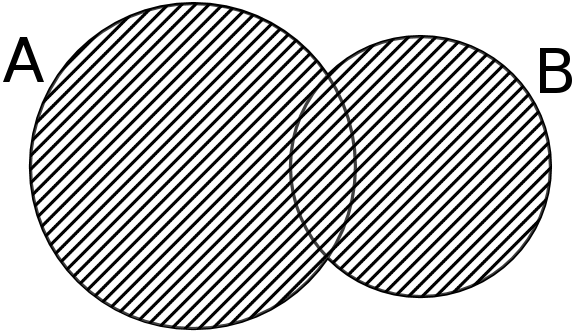
\includegraphics{images/pic3.png}
\end{minipage}

Рассмотрим примеры использования логических символов

\label{Problem1}
\underline{Задача №1}
Пусть A = \{квадратный трехчлен $y = ax^2 + bx +c$ принимает положительные значения при всех x\}, B = $\{\mathscr D < 0\}$, где $\mathscr D = b^2 -4ac$, C = $\{\mathscr D < 0, a>0\}=\{\mathscr D < 0\} \cap \{a>0\}$ Доказать, что $A \Rightarrow B, A \Leftrightarrow C.$
\begin{proof}
\begin{enumerate}
\item Предположим, что из A не следует B. Тогда $\mathscr D = b^2 - 4ac \geqslant 0$,  в этом сл-е квадратный трехчлен $y = ax^2 + bx + c$ имеет действительные корни $x_1$ и $x_2$ ($x_1 = x_2\ при\ \mathscr D = 0$) и поэтому обращается в нуль при $x= x_1$ и $x=x_2$, что противоречит A.
Итак, предположение о том, что из A не следует B, является неверным, поэтому из A следует B, т.е. $A \Rightarrow B$
\item Докажем, что $A \Rightarrow C$, воспользуемся равенством
\begin{equation}
y = a\left[ \left(x + \dfrac b{2a} \right)^2 - \dfrac{\mathscr D}{4a^2} \right]
\end{equation}
т.к. $A\Rightarrow {\mathscr D < 0}$, то выражение в квадратных скобках в формуле (1) положительно, и поэтому из условия $y > 0$ следуется, что $a>0$. Итак, $A\Rightarrow C$ \newline
Обратно: если имеет место $C$, т.е. $\mathscr D < 0$ и $a>0$, то из (1) следует, что $y > 0$ при всех (x). Таким образом, квадратный трехчлен $y = ax^2 +bx + c$ принимает положительные значения при всех
действительных значениях (x) тогда и только тогда, когда $a>0$ и $\mathscr D = b^2-4ac < 0$

\end{enumerate}
\end{proof}

\label{Problem2}
\underline{Задача №2} Пусть задано числовое множество $X$ и число $M$. Записать
с помощью кванторов отрицание утверждений:\newline
a) $A$=\{все элементы $x$ числового множества удовлетворяют условию $x<M$\}\newline
б) $B$=\{существует число $M>0$, такое, что все элементы $x$ из множества $X$ удовлетворяют условию $|x| \geqslant M$\}\newline
\textit{Решение:} 
а) Пусть $A$ не имеет места, т.е. не все элементы $x$ множества $X$
удовлетворяют условию $x<M$. Это означает, что найдется (существует) такой
элемент $x \in X$, для которого неравенство $x<M$ не выполняется, т.е. имеет
место противоположное неравенство $x \geqslant M$. (Если $A$ - высказывание, то
$\overline A$ - отрицание этого высказывания). Запишем $A$ и $\overline A$ с помощью кванторов\newline
$A$ = \{$\forall x \in X \rightarrow x < M$\}\newline
$\overline A$ = \{$\exists x \in X : x \geqslant M$\}  \newline
б) Пусть $B$ не имеет места, т.е. не существует числа $M>0$, такого, чтобы для
любого $x \in X$ имело место неравенство $|x| \geqslant M$. Это означает, что для
любого $M>0$ неравенство $|x| \geqslant M$ не может выполнятся для каждого $x \in X$.
Иначе говоря, существует такой элемент $x=x_M \in X$ (зависящий от $M$), для которого
неравенство не выполняется, т.е. справедливо неравенство $|x_M|<M$. С помощью кванторов
утверждения $B$ и $\overline B$ можно записать так:\newline
$B$ = \{$\exists M > 0 : \forall x \in X \rightarrow |x| \geqslant M$\}\newline
$\overline B$ = \{$\forall M > 0\ \exists x_M \in X : |x| < M$\}\newline

\label{Problem3}
\underline{Задача №3} Рассмотрим неопределенные высказывания, заданные на множестве
всех четырехугольников $Q$:\newline
$A(Q) \equiv $\{четырехугольник $Q$ - ромб\}; \newline
$B(Q) \equiv $\{диагонали четырехугольника $Q$ взаимно перпендикулярны\}. \newline
Доказать, что $\forall Q\ A(Q) \Rightarrow B(Q)$, а обратное утверждение 
$\forall Q\ B(Q) \Rightarrow A(Q)$ неверно.\newline
\textit{Решение:} 
Т.к. в любом ромбе диагонали взаимно перпендикулярны, то
$A(Q) \Rightarrow B(Q)$ для любого ромба $Q$. Обратная теорема неверна: существует
четырехугольник с взаимно перпендикулярными диагоналями, не являющийся ромбом.\newline

\label{Problem4}
\underline{Задача №4} Даны два предиката $P(x): x^2+x+1>0$ и $Q(x): x^2-4x+3=0$,
определенные на множестве $\mathbb R$. Установить, какие из высказываний истинны, 
а какие ложны: a) $\forall x\ P(x)$ б) $\exists x\ P(x)$ в) $\forall x\ Q(x)$ г) $\exists x\ Q(x)$.
(\textit{Замечание:} Предикат - это то, что утверждается о субъекте. Субъектом высказывания
называется то, о чем делается утверждение).\newline
\textit{Решение:}
Т.к. $x^2+x+1=\left (x+\dfrac12 \right)^2+\dfrac34 > 0$ при всех $x$, то будут
истинными высказывания $\forall x\ P(x)$ и $\exists x\ P(x)$. Т.к. $x^2-4x+3=0$ имеет 
только два действительных корня $x_1=3$ и $x_2=1$, то предикат $Q(x)$ принимает значение 1 только
при $x=3$ и \\$x=1$ и 0 в остальных случаях. Но тогда высказывание $\forall x\ Q(x)$ ложно, а
высказывание $\exists x\ Q(x)$ истинно.

\begin{center}
\large Упражнения
\end{center}
\label{Exercises}
\begin{enumerate}
	\item Доказать, что равенства: a) $A \cup B=B$ б) $A \cap B=A$ верны тогда и только тогда, когда $A \subset B$.
	\item Доказать, что равенства $A \setminus (B \setminus C)=(A \setminus B) \cup C$ верно тогда и только тогда когда, когда $A \supset C$.
	\item Доказать равенство:\newline
	\begin{minipage}{0,5\textwidth}
		а) $A \setminus (A \setminus B)=A \cap B$ \\
		б) $(A \setminus B) \cup (B \setminus A)=(A \cup B) \setminus (A \cap B)$
	\end{minipage}
	\begin{minipage}{0,5\textwidth}
		в) $(A \setminus B) \setminus C = A \setminus (B \cup C)$\\
		г) $(A \setminus B) \cap C = (A \cap C) \setminus (B \cap C)$
	\end{minipage}
	\item Доказать, что для любых высказываний $A$ и $B$ справедливы равенства
	$\overline {A \cap B}=\overline {A} \cup \overline {B}$ и $\overline {A \cup B}=\overline {A} \cap \overline {B}$
	\item Выяснить, какие из утверждений $A$ и $B$ следует из другого, используя символы <<$\Rightarrow$>>; <<$\Leftrightarrow$>>\newline
	a) $A \equiv $\{каждое из чисел $a$, $b$ делится на 7\}, $B \equiv $\{сумма $a$+$b$ делится на 7\} \\
	б) $A \equiv $\{последняя цифра числа $a$ четная\}, $B \equiv$\{число $a$ делится на 4\} \\
	в) Доказать, что квадратичная функция $y=ax^2+bx+c$ принимает отрицательные 
	значения при всех $x \in \mathbb R$ тогда и только тогда, когда $\mathscr D=b^2-4ac < 0$ и $a<0$.
	\item Пусть $f(x)=ax^2+bx+c\ (a \neq 0)$ - квадратный трехчлен. $\mathscr D=b^2-4ac$, $x_1$ и $x_2$ - корни
	квадратного трехчлена, $x_1 \leqslant x_2\ (\mathscr {D} \geqslant 0)$, $x_0=-\dfrac{b}{2a}$ - абсцисса вершины параболы
	$y=ax^2+bx+c$, $M$ и $K$ - заданные числа. Доказать, что: \\
	a) \{$x_1 < M,\ x_2 < M$\} $\Leftrightarrow$ \{$\mathscr {D} \geqslant 0,\ x_0<M,\ af(M)>0$\} \\
	б) \{$x_1 > M,\ x_2 < M$\} $\Leftrightarrow$ \{$\mathscr {D} \geqslant 0,\ x_0>M,\ af(M)>0$\} \\
	в) \{$x_1 < M < x_2$\} $\Leftrightarrow$ \{$af(M) < 0$\} \\
	г) \{$K < x_1 < M,\ K < x_2 < M$\} $\Leftrightarrow$ \{$\mathscr {D} \geqslant 0,\ K < x_0 < M,\ f(K)f(M)>0$\} \\
	д) \{$x_1 < K < M < x_2$\} $\Leftrightarrow$ \{$af(K)<0,\ af(M)<0$\}
\end{enumerate}
\end{document}
